\chapter{Pengenalan Kecerdasan Buatan dan Scikit-Learn}
\section{Kecerdasan Buatan}
\subsection{Definisi Kecerdasan Buatan}
    Kecerdasan Buatan biasa disebut dengan istilah AI (Artificial Intelligence). AI sendiri merupakan suatu cabang dalam bisnis sains komputer sains dimana mengkaji tentang bagaimana cara untuk menlengkapi sebuah komputer dengan kemampuan atau kepintaran layaknya atau mirip dengan yang dimiliki manusia. Sebagai contoh, sebagaimana komputer dapat berkomunikasi dengan pengguna baik menggunakan kata, suara maupun lain sebagainya. Dengan kemampuan ini, diharapkan komputer mampu mengambil keputusan sendiri untuk berbagai kasus yang ditemuinya kemudian itulah yang disebut dengan kecerdasan buatan. Kecerdasan buatan adalah kemampuan komputer digital atau robot yang dikendalikan konputer untuk melakukan tugas yang umumnya dikaitkan dengan sesuatu yang cerdas. Istilah ini sering diterapkan pada proyek pengembangan sistem yang diberkahi dengan karakteristik proses intelektual manusia, seperti kemampuan untuk berpikir, menemukan makna, menggeneralisasi, atau belajar dari pengalaman masa lalu.

    Kecerdasan Buatan adalah salah satu bidang studi yang berhubungan dengan pemanfaatan mesin untuk memecahkan persoalan yang rumit dengan cara lebih manusiawi dan lebih bisa di pahami oleh manusia. Kecerdasan buatan makin canggih dengan kemampuan komputer dalam memperbarui pengetahuannya dengan banyaknya testing dan perkembangan target analisa. Untuk kecerdasan buatan ada banyak contoh dan jenisnya. Salah satu contoh yang paling terkenal dari Artificial Intelligence ialah Google Assistant. Google Assistant digunakan untuk kemudahan user dalam menemukan berbagai hal maupun penyetingan langsung terhadap smartphone yang digunakan dan masih banyak lagi.

\subsection{Sejarah Kecerdasan Buatan}
    Artificial intelligence merupakan inovasi baru di bidang ilmu pengetahuan. Mulai terbentuk sejak adanya komputer modern dan kira-kira terjadi sekitaran tahun 1940 dan 1950. Ilmu pengetahuan komputer ini khusus ditujukan dalam perancangan otomatisasi tingkah laku cerdas dalam sistem kecerdasan komputer. Pada awal 50-an, studi tentang “mesin berpikir” memiliki berbagai nama seperti cybernetics, teori automata, dan pemrosesan innformasi. Pada tahun 1956, para ilmuan jenius seperti Alan Turing, Norbert, Wiener, Claude Shannon dan Warren McCullough telah bekerja secara independen dibidang cybernetics, matematika, algoritma dan teori jaringan. Namun, seprang ilmuan komputer dan kognitif John McCarthy adalah orang yang dating dengan ide untuk bergabung dengan upaya penelitian terpisah ini kedalam satu bidang yang akan mempelajari topic baru untuk imajinasi manusia yaitu kecerdasan buatan. Dia adalah orang yang menciptakan istilah tersebut dan kemudian mendirikan laboratorium Kecerdasan Buatan di MIT dan Stan ford.

    Pada tahun 1956, McCarthy yang sama mendirikan Konferensi Dartmouth di Hanover, New Hampshire. Peneliti terkemuka dalam teori kompleksitas, simulasi bahasa, hubungan antara keacakan dan pemikiran kreatif, jaringan saraf diundang. Tujuan dari bidang penelitian yang baru dibuat adalah untuk mengembangkan mesin yang dapat mensimulasikan setiap aspek kecerdasab. Itulah sebabnya Konferensi Dartmouth 1956 dianggap sebagai kelahiran Kecerdasan Buatan. Sejak saat itu, Kecerdasa Buatan telah hidup melalui decade kemuliaan dan cemoohan, yang dikenal luas sebagai musim panas dan musim dingin AI. Musim panasnya ditandai dengan optimism dan dana besar, sedangkan musim dinginnya dihadapkan dengan pemotongan dana, ketidakkpercayaan dan pesimisme.

\subsection{Perkembangan Kecerdasan Buatan}
    Teknologi Artificial Intelligence semakin ramai dibahas dalam berbagai diskusi teknologi di seluruh dunia.Menurut kebanyakan orang, pekerjaan seperti kasir, operator telepon, pengendara truk, dan lainnya sangat berpeluang besar untuk tergantikan oleh Artificial Intelligence. Mengapa terjadi hal demikian? dikarenakan memang bahwa AI lebih ungul dalam hal kinerja, fitur dan lain sebagainya. Namun, dalam beberapa aspek memang pekerja manusia masih unggul dibandingkan AI itu sendiri. Para generasi muda yang ada di dunia terutama di daerah Asia terlihat sudah memahami fungsi dan efek dari AI dalam kehidupan kita sehari-hari. Berdasarkan survei yang dilakukan oleh Microsoft, terdapat 39 persen responden yang mempertimbangkan untuk menggunakan mobil tanpa pengemudi dan 36 persen lainnya setuju bahwa robot masa depan dengan software untuk beroperasi mampu meningkatkan produktivitas. Dari survey tersebut kita sebagai pengguna AI harus lebih bijaksana dalam pengembangan dan penggunaan dari AI sehingga tanpa memberikan efek samping terhadap etos kerja dan keseharian kita sebagai pengguna dalam kehidupan sehari-hari.

    AI Summer 1 (1956-1973) KOnferensi Dartmounth diikuti oleh 17 tahun kemajuan luar biasa. Proyek penelitian yang dilakukan di MIT, universitas di Edinburgh, Stanford dan Carnegie Mellon menerima dana besar-besaran, yang akhirnya membuahkan hasil. Selama tahun-tahun itulah komputer pemrograman mulai melakukan masalah aljabar, membuktikan teorema geometris, memahami dan menggunakan sintaks dan tata bahasa Inggris. Terlepas dari ditinggalkannya koneksionisme dan terjemahan mesin yang gagal, yang menunda penelitian Natural Language Processing (NLP) selama bertahun-tahun, banyak prestasi dari masa lalu yang membuat sejarah. Berikut ini beberapa diantaranya : Pelopor pembelajaran mesin, Ray Solomonoff meletakkan dasar-dasar teori metematika AI, memperkenalkan metode Bayesian universal untuk inferensi dan preddiksi induktif Thomas Evans menciptakan program ANALOGI heuristik, yang memungkinkan komputer memecahkan masalah geometri-analogi Unimation, perusahaan robotika pertma didunia, menciptakan robot industri Unimate, yang bekerja pada jalur perakitan modil Genenral Motors. Joseph Weizenbaum membangun ELIZA-program interaktif yang dapat membawa percakapan dalam bahasan Inggris tentang topik apapun. Ross Quillian menunjukkan jaring semanik, sedangkan Jaime Carbonell (Sr.) mengembangkan Cendikia-program interaktif untuk instruksi yang dibantu komputer berdasarkan jaring semantik. Edward Feigenbaum dan Julian Feldman menerbitkan Computeks and Thought, kumpulan artikel pertama tentang AI.

\section{Scikit-Learn}
\subsection{Supervised Learning}
Supervised Learning adalah tugas pengumpulan data untuk menyimpulkan fungsi dari data pelatihan berlabel. Data pelatihan terdiri dari serangkaian contoh pelatihan. Dalam supervised learning, setiap contoh adalah pasangan yang terdiri dari objek input (biasanya vektor) dan nilai output yang diinginkan(juga disebut sinyal pengawasan super). Algoritma pembelajaran yang diawasi menganalisis data pelatihan dan menghasilkan fungsi yang disimpulkan, yang dapat digunakan untuk memetakan contoh-contoh baru. Skenario optimal akan memungkinkan algoritma menentukan label kelas dengan benar untuk instance yang tidak terlihat. Ini membutuhkan algoritma pembelajaran untuk menggeneralisasi dari data pelatihan untuk situasi yang tidak terlihat dengan cara yang "masuk akal". Supervised Learning adalah pendekatan dimana sudah terdapat data yang dilatih selain itu juga terdapat variable yang ditargetkan sehingga tujuan dari pendekatan ini yaitu mengelompokkan suatu data ke dta yang sudah ada. Supervised Learning menyediakan algoritma pembelajaran dengan jumlah yang diketahui untuk mendukung penilaian dimasa depan. Chatbots, mobil self-driving, program pengenalan wajah, sistem pakar dan robot adalah beberapa sistem yang dapat menggunakan pembelajaran yang diawasi atau tidak diawasi. Supervised Learning sebagian besar terkait dengan AI berbasis pengambilan tetapi mereka juga mungkin mampu menggunakan model pembelajaran generatif. Data pelatihan untuk pembelajaran yang diawasi mencakup serangkaian contoh dengan subjek input berpasangan dan output yang diinginkan (yang juga disebut sebagai sinyal pengawasan).

Dalam pembelajaran yang diawasi untuk pemrosesan gambar, misalnya sistem AI mungkin dilengkapi dengan gambar berlabel kendaraan dalam ketegori seperti mobil dan truk. Setelah jumlah pengamatan yang cukup, sistem harus dapat membedakan antara dan mengkategorikan gambar yang tidak berlabel, dimana waktu pelatihan dapat dikatakan lengkap. Model Supervised Learning memiliki beberapa keunggulan dibandingkan pendekatan tanpa pengawasan, tetapi mereka juga memiliki keterbatasan. Sistem lebih cenderung membuat penilaian bahwa manusia dapat berhubungan, misalnya karena manusia telah memberikan dasar untuk keputusan. Namun, dalam kasus metode berbasis pengambilan, Supervised Learning mengalami kesulitan dalam menangani informaasi baru. Jika suatu sistem dengan kategori untuk mobil dan truk disajikan dengan sepeda, misalnya ia harus salah dikelompokkan dalam satu kategori ata yang lain. Namun. jika sistem AI bersifat generatif, ia mungkin tidak tahu apa sepeda itu tetapi akan dapat mengenalinya sebagai milik kategori yang terpisah.

\subsection{Regresi}
Regresi adalah metode analisis statistik yang digunakan untuk melihat pengaruh antara dua ataupun lebih variabel. Regresi adalah membahas masalah ketika variabel output adalah nilai riil atau berkelanjutan, seperti "gaji" atau "berat". Banyak model yang berbeda dapat digunakan makan, yang paling sederhana adalah regresi linier. Ia mencoba untuk menyesuaikan data dengan hyper-plane terbaik yang melewati poin.

\subsection{Klasifikasi}
Klasifikasi adalah pembagian sesuatu menurut kelas-kelas ( class ). Menurut Ilmu Pengetahuan, Klasifikasi merupakan proses pengelompokkan benda berdasarkan ciri-ciri persamaan dan juga perbedaan. Dalam masalah klasifikasi, kami mencoba memprediksi sejumlah nilai terpisah. Label (y) umumnya datang dalam bentuk kategorikal dan mewakili sejumlah kelas. Dalam pembelajaran mesin dan statistik, klasifikasi adalah pendekatan pembelajaran yang diawasi di mana program komputer belajar dari input data yang diberikan kepadanya dan kemudian menggunakan pembelajaran ini untuk mengklasifikasikan pengamatan baru. Kumpulan data ini mungkin hanya bersifat dua kelas (seperti mengidentifikasi apakah orang tersebut berjenis kelamin laki-laki atau perempuan atau bahwa surat itu spam atau bukan-spam) atau mungkin juga multi-kelas. Beberapa contoh masalah klasifikasi adalah: pengenalan ucapan, pengenalan tulisan tangan, identifikasi metrik, klasifikasi dokumen dll.

\subsection{Unsupervised Learning}
Unsupervised Learning berbeda dengan Supervised Leraning. Perbedaannya ialah unsupervised learning tidak memiliki data latih, sehingga dari data yang ada kita mengelompokan data tersebut menjadi 2 ataupun 3 bagian dan seterusnya. Unsupervised Learning adalah pelatihan algoritma kecerdasan buatan (AI) menggunakan informasi yang tidak diklasifikasikan atau diberi label dan memungkinkan algoritma untuk bertindak atas informasi tersebut tanpa bimbingan. Dalam Unsupervised Learning, sistem AI dapat mengelompokkan informasi yang tidak disortir berdasarkan persamaan dan perbedaan meskipun tidak ada kategori yang disediakan.

Dalam Unsupervised Learning, sistem AI disajikan dengan data yang tidak berlabel, tidak terkategorisasi dan algoritma sistem bekerja pada data tanpa pelatihan sebelumnya. Outputnya tergantung pada algoritma kode. Menundukkan suatu sistem pada Unsupervised Learning adalah salah satu cara untuk menguji AI. Algoritma Unsupervised Learning dapat melakukan tugas pemrosesan yang lebih kompleks daripada sistem pembelajaran yang
diawasi. Namun, pembelajaran tanpa pengawasan bisa lebih tidak terduga daripada model alternatif. Sementara Unsupervised Learningi mungkin, misalnya, mencari tahu sendiri cara memilah kucing dari anjing, mungkin juga menambahkan kategori yang tidak terduga dan tidak diinginkan untuk menangani breed yang tidak biasa, membuat kekacauan bukannya keteraturan

\subsection{Data Set}
Dataset adalah objek yang merepresentasikan data dan juga relasi yang ada di memory. Strukturnya mirip dengan data di database, namun bedanya
dataset berisi koleksi dari data table dan data relation. mendapatkan data yang tepat berarti mengumpulkan atau mengidentifikasi data yang berkorelasi dengan hasil yang ingin Anda prediksi; yaitu data yang berisi sinyal tentang peristiwa yang Anda pedulikan. Data harus diselaraskan dengan masalah yang Anda coba selesaikan. Gambar kucing tidak terlalu berguna ketika Anda sedang membangun sistem identifikasi wajah. Memverifikasi bahwa data selaras dengan masalah yang ingin Anda selesaikan harus dilakukan oleh ilmuwan data. Jika Anda tidak memiliki data yang tepat, maka upaya Anda untuk membangun solusi AI harus kembali ke tahap pengumpulan data. Format ujung kanan untuk pembelajaran dalam umumnya adalah tensor, atau array multi-dimensi. Jadi jalur pipa data yang dibangun untuk pembelajaran mendalam umumnya akan mengkonversi semua data - baik itu gambar, video, suara, suara, teks atau deret waktu  menjadi vektor dan tensor yang dapat diterapkan operasi aljabar linier. Data itu seringkali perlu dinormalisasi, distandarisasi dan dibersihkan untuk meningkatkan kegunaannya, dan itu semua adalah langkah dalam ETL pembelajaran mesin. Deeplearning4j menawarkan alat ETV DataVec untuk melakukan tugas-tugas pemrosesan data tersebut.

Pembelajaran yang dalam, dan pembelajaran mesin yang lebih umum, membutuhkan pelatihan yang baik agar bekerja dengan baik. Mengumpulkan dan membangun set pelatihan  badan yang cukup besar dari data yang diketahui  membutuhkan waktu dan pengetahuan khusus domain tentang di mana dan bagaimana mengumpulkan informasi yang relevan. Perangkat pelatihan bertindak sebagai tolok ukur terhadap mana jaring pembelajaran dalam dilatih. Itulah yang mereka pelajari untuk direkonstruksi sebelum mereka melepaskan data yang belum pernah mereka lihat sebelumnya. Pada tahap ini, manusia yang berpengetahuan luas perlu menemukan data mentah yang tepat dan mengubahnya menjadi representasi numerik yang dapat dipahami oleh algoritma pembelajaran mendalam, tensor. Membangun set pelatihan, dalam arti tertentu, pra-pra pelatihan. Set pelatihan yang membutuhkan banyak waktu atau keahlian dapat berfungsi sebagai keunggulan dalam dunia ilmu data dan pemecahan masalah. Sifat keahlian sebagian besar dalam memberi tahu algoritma Anda apa yang penting bagi Anda dengan memilih apa yang masuk ke dalam set pelatihan. Ini melibatkan menceritakan sebuah kisah  melalui data awal yang Anda pilih yang akan memandu jaring pembelajaran mendalam Anda saat mereka mengekstraksi fitur-fitur penting, baik di set pelatihan maupun dalam data mentah yang telah mereka ciptakan untuk dipelajari. Untuk membuat set pelatihan yang bermanfaat, Anda harus memahami masalah yang Anda selesaikan; yaitu apa yang Anda inginkan agar jaring pembelajaran mendalam Anda memperhatikan, di mana hasil yang ingin Anda prediksi.

\subsection{Training Set}
Training Set adalah set digunakan oleh algoritma klassifikasi . Dapat dicontohkan dengan : decision tree, bayesian, neural network dll. Semuanya dapat digunakan untuk membentuk sebuah model classifier. Menjalankan pelatihan yang diatur melalui jaringan saraf mengajarkan pada net
cara menimbang berbagai fitur, menyesuaikan koefisien berdasarkan kemungkinan mereka meminimalkan kesalahan dalam hasil Anda. Koefisien-koefisien tersebut, juga dikenal sebagai parameter, akan terkandung dalam tensor dan bersama-sama mereka disebut model, karena mereka mengkodekan model data yang mereka latih. Mereka adalah takeaways paling penting yang akan Anda dapatkan dari pelatihan jaringan saraf.

\subsection{Testing Set}
Testing Set adalah set yang digunakan untuk mengukur sejauh mana classifier berhasil melakukan klasifikasi dengan benar. Ini berfungsi sebagai meterai persetujuan, dan Anda tidak menggunakannya sampai akhir. Setelah Anda melatih dan mengoptimalkan data Anda, Anda menguji jaringan saraf Anda terhadap pengambilan sampel acak akhir ini. Hasil yang dihasilkannya harus memvalidasi bahwa jaring Anda secara akurat mengenali gambar, atau mengenalinya setidaknya [x] dari jumlah tersebut. Jika Anda tidak mendapatkan prediksi yang akurat, kembalilah ke set pelatihan, lihat hyperparameter yang Anda gunakan untuk menyetel jaringan, serta kualitas data Anda dan lihat teknik pra-pemrosesan Anda.

\section{Instalasi dan Pemakaian Scikit-Learn}
\subsection{Instalasi library scikit dari anaconda, mencoba kompilasi dan uji coba ambil contoh kode dan lihat variabel explorer}
\begin{enumerate}
\item Pastikan bahwa sudah terinstal Anaconda pada PC anda, caranya buka CMD lalu ketikan \textit{conda --version} jika hasilnya seperti
\begin{figure}
	\begin{center}
   	 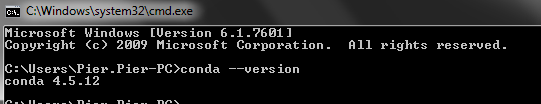
\includegraphics[scale=0.5]{figures/versiconda.png}
   	 \caption{Versi Anaconda Yang Digunakan}	
	\end{center}
\end{figure}

\item Pastikan juga Kebutuhan Scikit seperti Numpy, Scipy dan Python telah terinstal. untuk mengeceknya buka CMD dan ketikan seperti gambar berikut.
\begin{figure}
	\begin{center}
   	 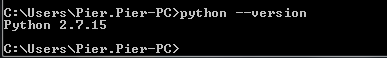
\includegraphics[scale=0.5]{figures/gambar.png}
   	 \caption{Versi Python Yang Digunakan}	
	\end{center}
\end{figure}

\item Pada CMD ketikan \textit{conda install scikit-learn} kemudian tunggu sampai instalasi selesai.
\begin{figure}[!htbp]
	\begin{center}
   	 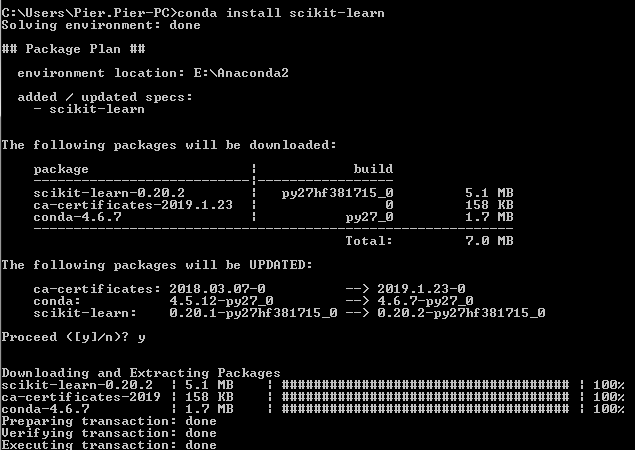
\includegraphics[scale=0.5]{figures/instalscikit.png}
   	 \caption{Instalasi Scikit Dari Anaconda}	
	\end{center}
\end{figure}

\item Setelah itu, kita akan mencoba salah satu contoh dasar penggunaan scikit pada website sebelumnya. Dan disini menggunakan contoh Multilabel classification.
\item Salin skrip contoh tersebut ke Text Editor Visual Code atau yang anda miliki. File ini kemudian di save dengan nama `contoh.py'
\begin{figure}
	\begin{center}
   	 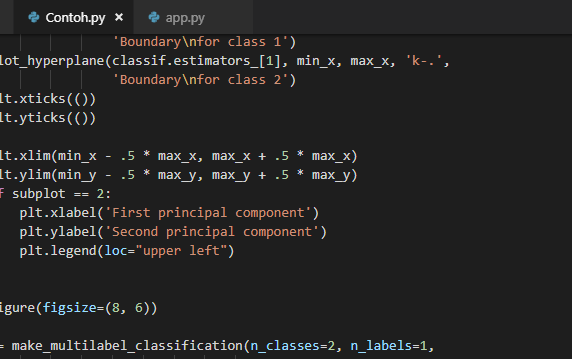
\includegraphics[scale=0.5]{figures/contoh.png}
   	 \caption{Contoh Skrip}	
	\end{center}
\end{figure}
\item Setelah tersimpan, jalankan di CMD dengan mengetikan `python contoh.py' maka akan muncul hasil seperti dibawah ini.
\begin{figure}
	\begin{center}
   	 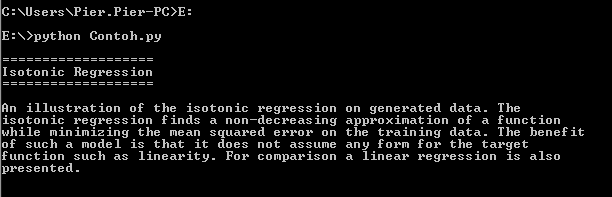
\includegraphics[scale=0.5]{figures/hasil1.png}
   	 \caption{Hasil Yang Muncul Di CMD}	
	\end{center}
\end{figure}

\begin{figure}
	\begin{center}
   	 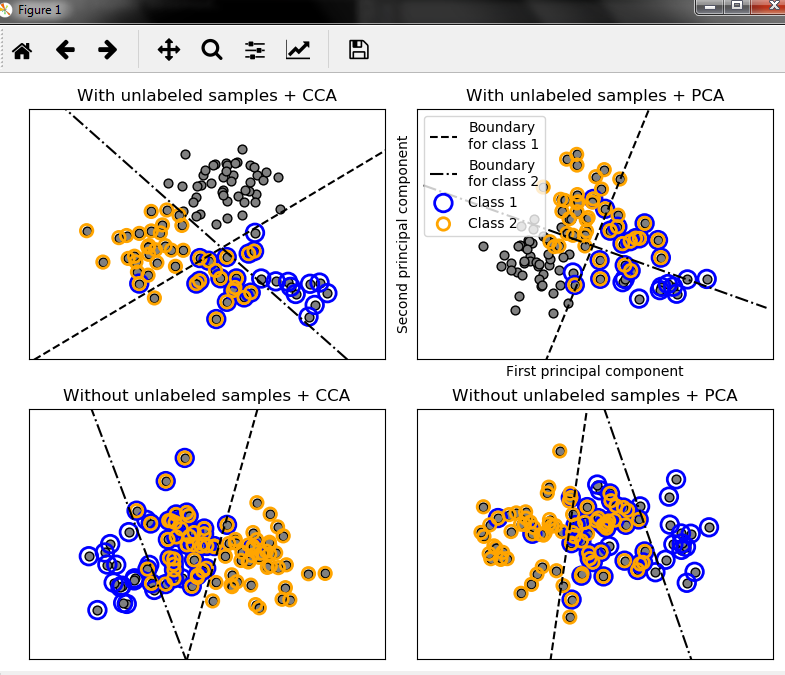
\includegraphics[scale=0.5]{figures/hasil2.png}
   	 \caption{Gambar Yang Muncul Dari Matplotlib}	
	\end{center}
\end{figure}
\end{enumerate}

\subsection{Loading an example dataset}

\begin{enumerate}
\item Mengimmport dataset, iris dan digit sebagai contoh data.
\begin{figure}
	\begin{center}
   	 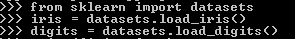
\includegraphics[scale=0.5]{figures/penjelasan1.png}
   	 \caption{Penjelasan }	
	\end{center}
\end{figure}
\item Misalnya, dalam kasus dataset digit, digits.data memberikan akses ke fitur yang dapat digunakan untuk mengklasifikasikan sampel digit.
\begin{figure}
	\begin{center}
   	 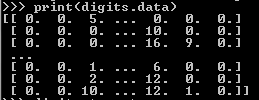
\includegraphics[scale=0.5]{figures/penjelasan2.png}
   	 \caption{Penjelasan 2}	
	\end{center}
\end{figure}
\item Digit.target memberikan kebenaran dasar untuk dataset digit, yaitu angka yang sesuai dengan setiap gambar digit yang dipelajari.
\begin{figure}
	\begin{center}
   	 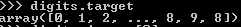
\includegraphics[scale=0.5]{figures/penjelasan3.png}
   	 \caption{Penjelasan 3}	
	\end{center}
\end{figure}
\item Menggambarkan bagaimana mulai dari masalah awal seseorang dapat membentuk data untuk konsumsi di scikit-belajar.
\begin{figure}
	\begin{center}
   	 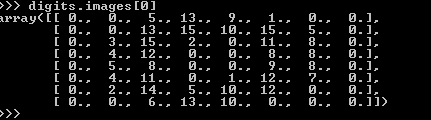
\includegraphics[scale=0.5]{figures/penjelasan4.png}
   	 \caption{Penjelasan 4}	
	\end{center}
\end{figure}

\end{enumerate}

\subsection{Learning and predicting}
\begin{enumerate}
\item Pada website sebelumnya, cari Learning And Predicting dan ikuti langkah -langkahnya.
\item Buka Python Shell, atau dengan membukan Command Prompt di PC dan mengetikan python. maka akan masuk ke Python Shellnya pada gambar\ref{gambar1}.
\begin{figure}
	\begin{center}
   	 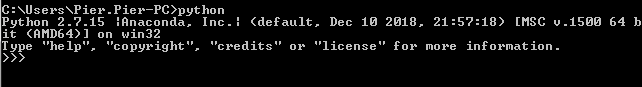
\includegraphics[scale=0.5]{figures/tasya1.png}
   	 \caption{Membuka Python Shell}
   	 \label{gambar1}
	\end{center}
\end{figure}

\item Pada python shell ketikan (from sklearn import svm) yang dimana artinya akan memanggil dan menggunakan estimator dari kelas sklearn.svm.SVC pada gambar\ref{gambar2}.
\begin{figure}
	\begin{center}
   	 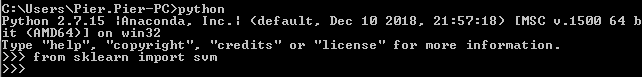
\includegraphics[scale=0.5]{figures/tasya2.png}
   	 \caption{Menggunakan Estimator Sklearn}
     \label{gambar2}	
	\end{center}
\end{figure}

\item Kemudian, kita definisikan clf sebagai classfier, disini gamma didefinisikan secara manual pada gambar\ref{gambar3}.
\begin{figure}
	\begin{center}
   	 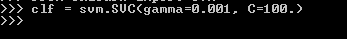
\includegraphics[scale=1]{figures/tasya3.png}
   	 \caption{Mendefinisikan Classifier}
     \label{gambar3}	
	\end{center}
\end{figure}

\item Estimator clf (for classifier) pertama kali dipasang pada model. Ini dilakukan dengan melewati training set ke metode fit. Untuk training set, akan menggunakan semua gambar dari set data yang ada, kecuali untuk gambar terakhir, yang dicadangan untuk prediksi. Pada skrip dibawah memilih training set dengan sintaks Python [: -1], yang menghasilkan array baru yang berisi semua kecuali item terakhir dari digits.data terlihat pada gambar\ref{gambar4}.
\begin{figure}
	\begin{center}
   	 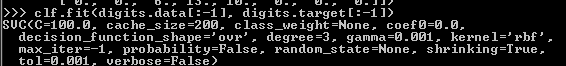
\includegraphics[scale=0.5]{figures/tasya4.png}
   	 \caption{Memanggil Classifier Tanpa Baris Terakhir}
     \label{gambar4}	
	\end{center}
\end{figure}

\item Pada penggalan skrip dibawah, ini menunjukan prediksi nilai baru menggunakan gambar terakhir dari digits.data. Dengan prediksi akan menentukan gambar dari set pelatihan yang paling cocok dengan gambar terakhir terlihat pada gambar\ref{gambar5}.
\begin{figure}
	\begin{center}
   	 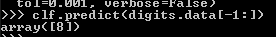
\includegraphics[scale=1]{figures/tasya5.png}
   	 \caption{Memprediksi Nilai Baru}
     \label{gambar5}	
	\end{center}
\end{figure}
\end{enumerate}